% Options for packages loaded elsewhere
\PassOptionsToPackage{unicode}{hyperref}
\PassOptionsToPackage{hyphens}{url}
%
\documentclass[
]{article}
\usepackage{lmodern}
\usepackage{amssymb,amsmath}
\usepackage{ifxetex,ifluatex}
\ifnum 0\ifxetex 1\fi\ifluatex 1\fi=0 % if pdftex
  \usepackage[T1]{fontenc}
  \usepackage[utf8]{inputenc}
  \usepackage{textcomp} % provide euro and other symbols
\else % if luatex or xetex
  \usepackage{unicode-math}
  \defaultfontfeatures{Scale=MatchLowercase}
  \defaultfontfeatures[\rmfamily]{Ligatures=TeX,Scale=1}
\fi
% Use upquote if available, for straight quotes in verbatim environments
\IfFileExists{upquote.sty}{\usepackage{upquote}}{}
\IfFileExists{microtype.sty}{% use microtype if available
  \usepackage[]{microtype}
  \UseMicrotypeSet[protrusion]{basicmath} % disable protrusion for tt fonts
}{}
\makeatletter
\@ifundefined{KOMAClassName}{% if non-KOMA class
  \IfFileExists{parskip.sty}{%
    \usepackage{parskip}
  }{% else
    \setlength{\parindent}{0pt}
    \setlength{\parskip}{6pt plus 2pt minus 1pt}}
}{% if KOMA class
  \KOMAoptions{parskip=half}}
\makeatother
\usepackage{xcolor}
\IfFileExists{xurl.sty}{\usepackage{xurl}}{} % add URL line breaks if available
\IfFileExists{bookmark.sty}{\usepackage{bookmark}}{\usepackage{hyperref}}
\hypersetup{
  pdftitle={Outcome Inequalty by Race in Early Stage High Grade Serous Ovarian Cancer},
  pdfauthor={Kevin Kremer},
  hidelinks,
  pdfcreator={LaTeX via pandoc}}
\urlstyle{same} % disable monospaced font for URLs
\usepackage[margin=1in]{geometry}
\usepackage{graphicx,grffile}
\makeatletter
\def\maxwidth{\ifdim\Gin@nat@width>\linewidth\linewidth\else\Gin@nat@width\fi}
\def\maxheight{\ifdim\Gin@nat@height>\textheight\textheight\else\Gin@nat@height\fi}
\makeatother
% Scale images if necessary, so that they will not overflow the page
% margins by default, and it is still possible to overwrite the defaults
% using explicit options in \includegraphics[width, height, ...]{}
\setkeys{Gin}{width=\maxwidth,height=\maxheight,keepaspectratio}
% Set default figure placement to htbp
\makeatletter
\def\fps@figure{htbp}
\makeatother
\setlength{\emergencystretch}{3em} % prevent overfull lines
\providecommand{\tightlist}{%
  \setlength{\itemsep}{0pt}\setlength{\parskip}{0pt}}
\setcounter{secnumdepth}{-\maxdimen} % remove section numbering
\usepackage{booktabs}
\usepackage{longtable}
\usepackage{array}
\usepackage{multirow}
\usepackage{wrapfig}
\usepackage{float}
\usepackage{colortbl}
\usepackage{pdflscape}
\usepackage{tabu}
\usepackage{threeparttable}
\usepackage{threeparttablex}
\usepackage[normalem]{ulem}
\usepackage{makecell}
\usepackage{xcolor}

\title{Outcome Inequalty by Race in Early Stage High Grade Serous Ovarian
Cancer}
\author{Kevin Kremer}
\date{02/23/21}

\begin{document}
\maketitle

\hypertarget{survival-of-early-stage-hgsoc-by-race}{%
\section{Survival of early-stage HGSOC by
race}\label{survival-of-early-stage-hgsoc-by-race}}

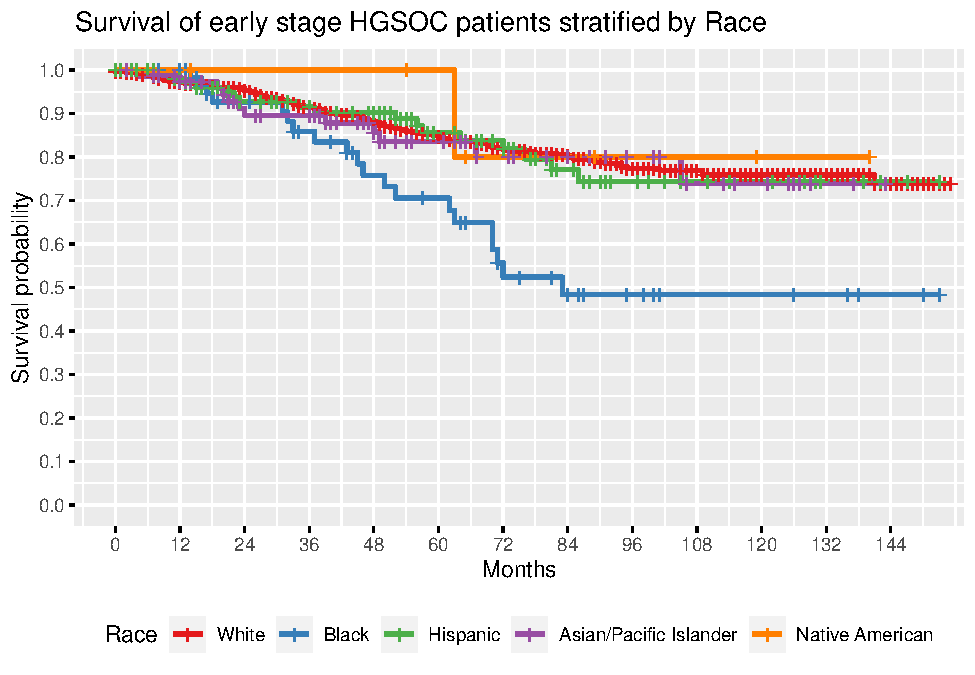
\includegraphics{EarlyOvaryRace_files/figure-latex/unnamed-chunk-1-1.pdf}

\begin{verbatim}
## 
##  Pairwise comparisons using Log-Rank test 
## 
## data:  HGS.ES and Race 
## 
##          White   Black   Hispanic API    
## Black    0.00099 -       -        -      
## Hispanic 0.88561 0.03049 -        -      
## API      0.88561 0.08697 0.88561  -      
## Native   0.88561 0.51590 0.88561  0.88561
## 
## P value adjustment method: BH
\end{verbatim}

\begin{tabular}[t]{l|r}
\hline
Race & Count\\
\hline
White & 795\\
\hline
Black & 60\\
\hline
Hispanic & 111\\
\hline
API & 76\\
\hline
Native & 7\\
\hline
\end{tabular}

\hypertarget{comparing-black-race-to-all-other-races-combined}{%
\section{Comparing Black Race to All Other Races
Combined}\label{comparing-black-race-to-all-other-races-combined}}

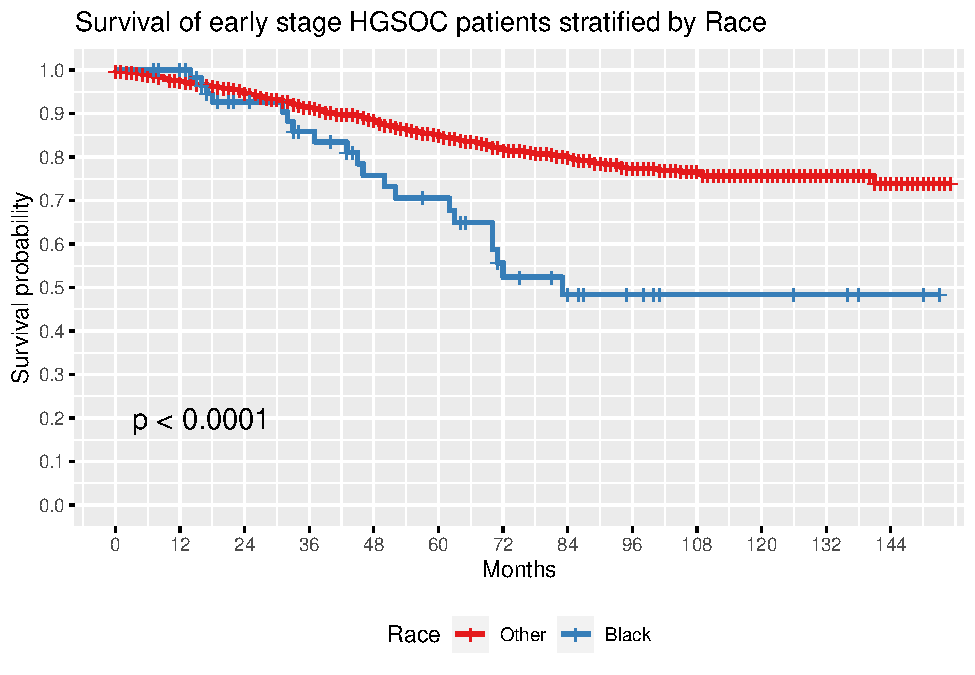
\includegraphics{EarlyOvaryRace_files/figure-latex/unnamed-chunk-2-1.pdf}

\begin{tabular}[t]{l|r}
\hline
Black Race & Count\\
\hline
no & 992\\
\hline
yes & 60\\
\hline
\end{tabular}

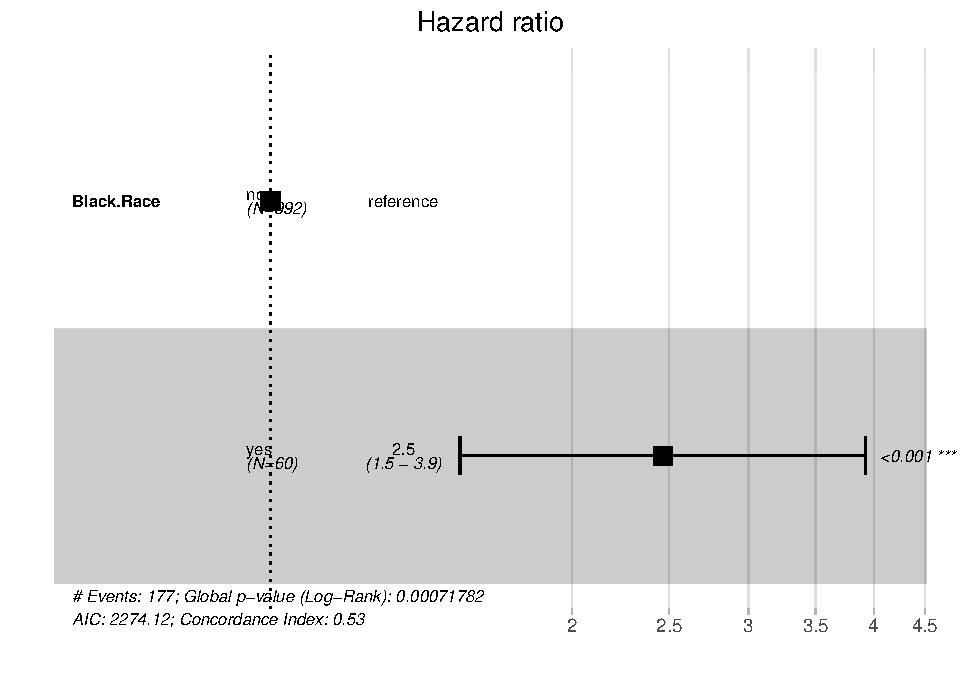
\includegraphics{EarlyOvaryRace_files/figure-latex/unnamed-chunk-3-1.pdf}

\begin{verbatim}
## Call:
## coxph(formula = Surv(SurvMonths, COD) ~ Black.Race, data = HGS.ES)
## 
##   n= 1052, number of events= 177 
## 
##                 coef exp(coef) se(coef)     z Pr(>|z|)    
## Black.Raceyes 0.9013    2.4628   0.2377 3.792  0.00015 ***
## ---
## Signif. codes:  0 '***' 0.001 '**' 0.01 '*' 0.05 '.' 0.1 ' ' 1
## 
##               exp(coef) exp(-coef) lower .95 upper .95
## Black.Raceyes     2.463      0.406     1.546     3.924
## 
## Concordance= 0.527  (se = 0.011 )
## Likelihood ratio test= 11.44  on 1 df,   p=7e-04
## Wald test            = 14.38  on 1 df,   p=1e-04
## Score (logrank) test = 15.38  on 1 df,   p=9e-05
\end{verbatim}

\hypertarget{comparing-black-race-to-white-race}{%
\section{Comparing Black Race to White
Race}\label{comparing-black-race-to-white-race}}

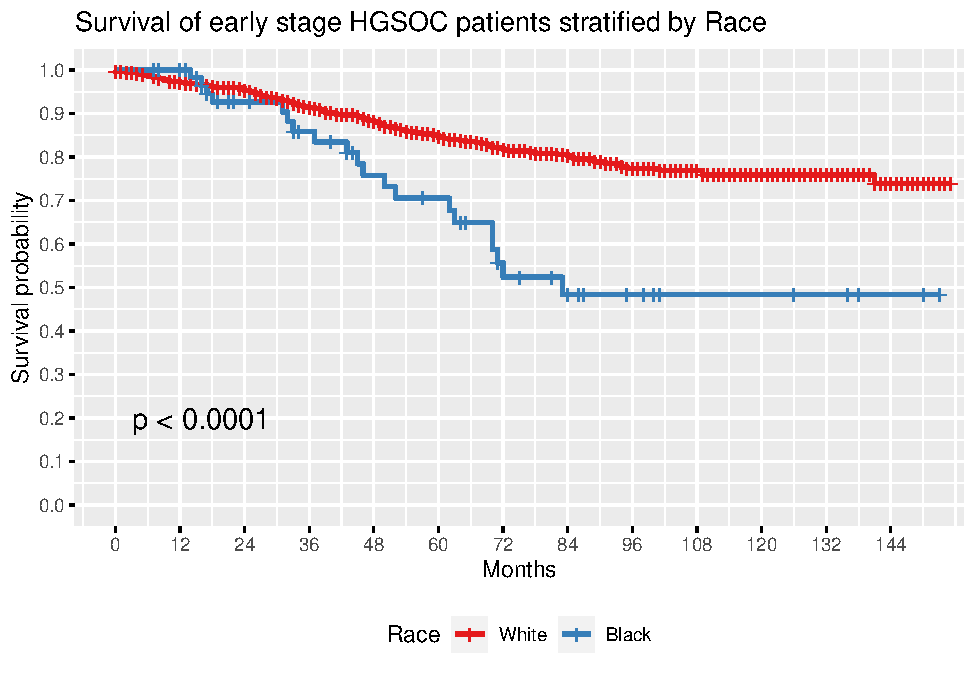
\includegraphics{EarlyOvaryRace_files/figure-latex/unnamed-chunk-4-1.pdf}

\begin{tabular}[t]{l|r}
\hline
Race & Count\\
\hline
White & 795\\
\hline
Black & 60\\
\hline
\end{tabular}

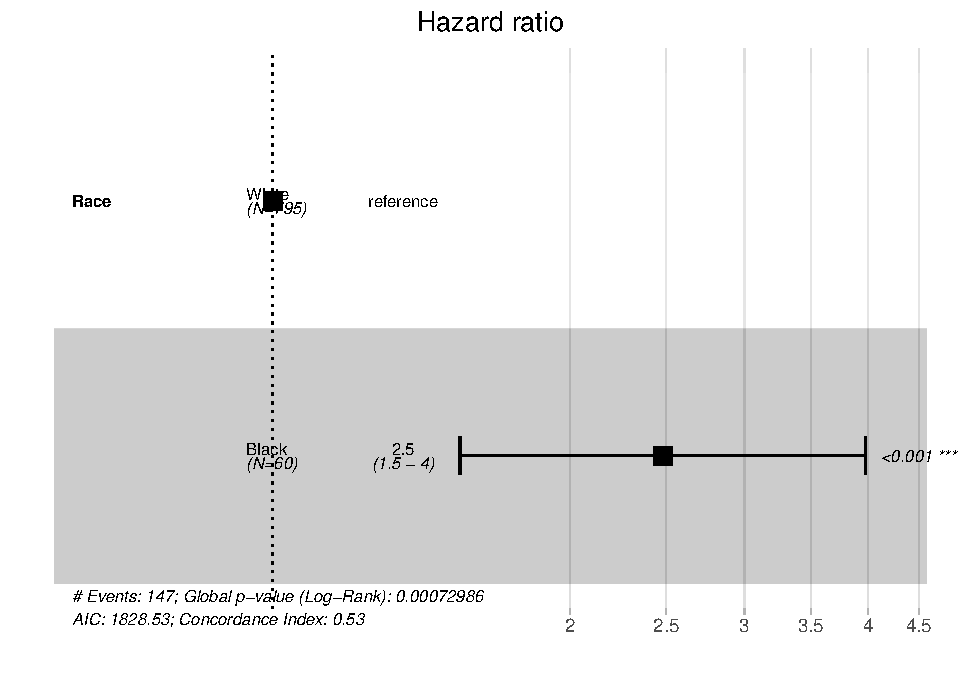
\includegraphics{EarlyOvaryRace_files/figure-latex/unnamed-chunk-5-1.pdf}

\begin{verbatim}
## Call:
## coxph(formula = Surv(SurvMonths, COD) ~ Race, data = HGS.WB)
## 
##   n= 855, number of events= 147 
## 
##             coef exp(coef) se(coef)    z Pr(>|z|)    
## RaceBlack 0.9082    2.4798   0.2409 3.77 0.000164 ***
## ---
## Signif. codes:  0 '***' 0.001 '**' 0.01 '*' 0.05 '.' 0.1 ' ' 1
## 
##           exp(coef) exp(-coef) lower .95 upper .95
## RaceBlack      2.48     0.4033     1.546     3.977
## 
## Concordance= 0.533  (se = 0.013 )
## Likelihood ratio test= 11.41  on 1 df,   p=7e-04
## Wald test            = 14.21  on 1 df,   p=2e-04
## Score (logrank) test = 15.21  on 1 df,   p=1e-04
\end{verbatim}

\hypertarget{comparing-black-race-to-hispanic-race}{%
\section{Comparing Black Race to Hispanic
Race}\label{comparing-black-race-to-hispanic-race}}

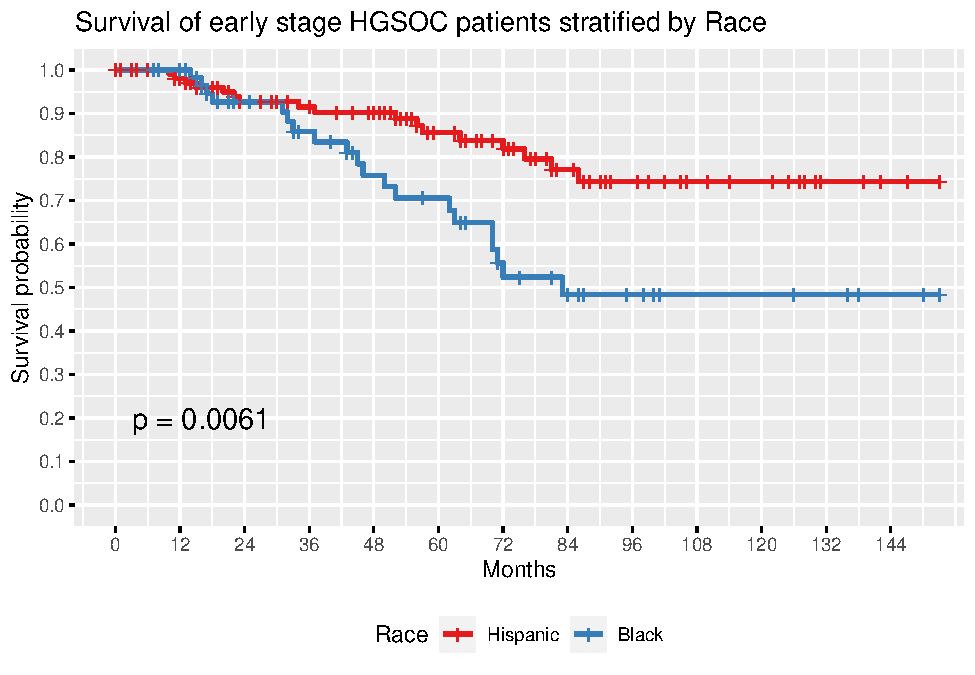
\includegraphics{EarlyOvaryRace_files/figure-latex/unnamed-chunk-6-1.pdf}

\begin{tabular}[t]{l|r}
\hline
Race & Count\\
\hline
Hispanic & 111\\
\hline
Black & 60\\
\hline
\end{tabular}

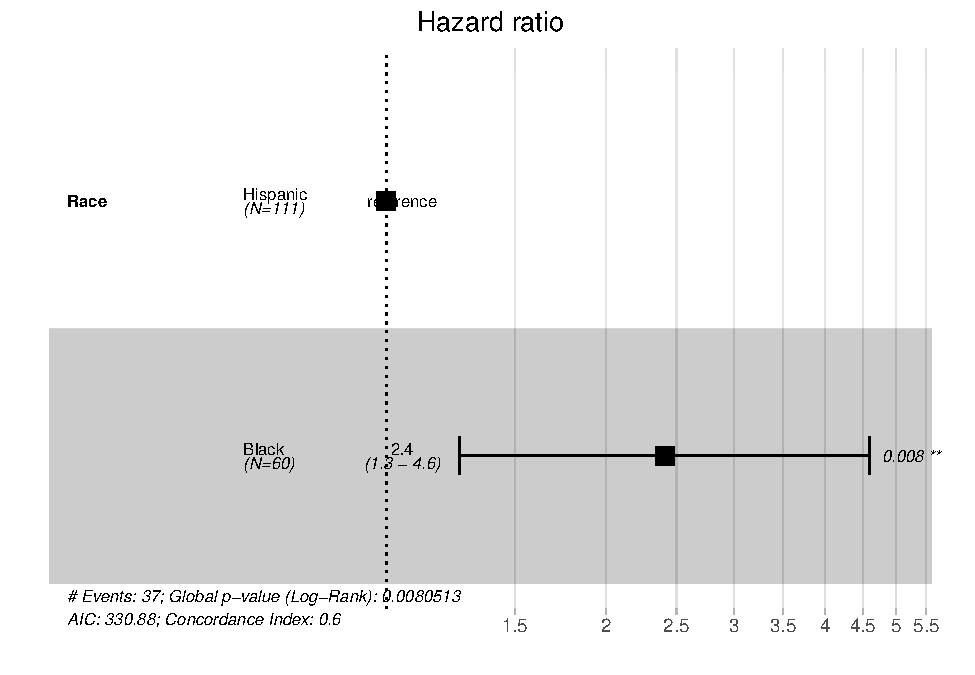
\includegraphics{EarlyOvaryRace_files/figure-latex/unnamed-chunk-7-1.pdf}

\begin{verbatim}
## Call:
## coxph(formula = Surv(SurvMonths, COD) ~ Race, data = HGS.HB)
## 
##   n= 171, number of events= 37 
## 
##             coef exp(coef) se(coef)    z Pr(>|z|)   
## RaceBlack 0.8791    2.4088   0.3304 2.66  0.00781 **
## ---
## Signif. codes:  0 '***' 0.001 '**' 0.01 '*' 0.05 '.' 0.1 ' ' 1
## 
##           exp(coef) exp(-coef) lower .95 upper .95
## RaceBlack     2.409     0.4152      1.26     4.603
## 
## Concordance= 0.596  (se = 0.044 )
## Likelihood ratio test= 7.02  on 1 df,   p=0.008
## Wald test            = 7.08  on 1 df,   p=0.008
## Score (logrank) test = 7.54  on 1 df,   p=0.006
\end{verbatim}

\hypertarget{does-the-addition-of-chemotherapy-in-patients-with-unknown-nodal-status-improve-outcomes-in-different-races}{%
\section{Does the addition of chemotherapy in patients with unknown
nodal status improve outcomes in different
races?}\label{does-the-addition-of-chemotherapy-in-patients-with-unknown-nodal-status-improve-outcomes-in-different-races}}

\hypertarget{black-race}{%
\subsection{Black Race}\label{black-race}}

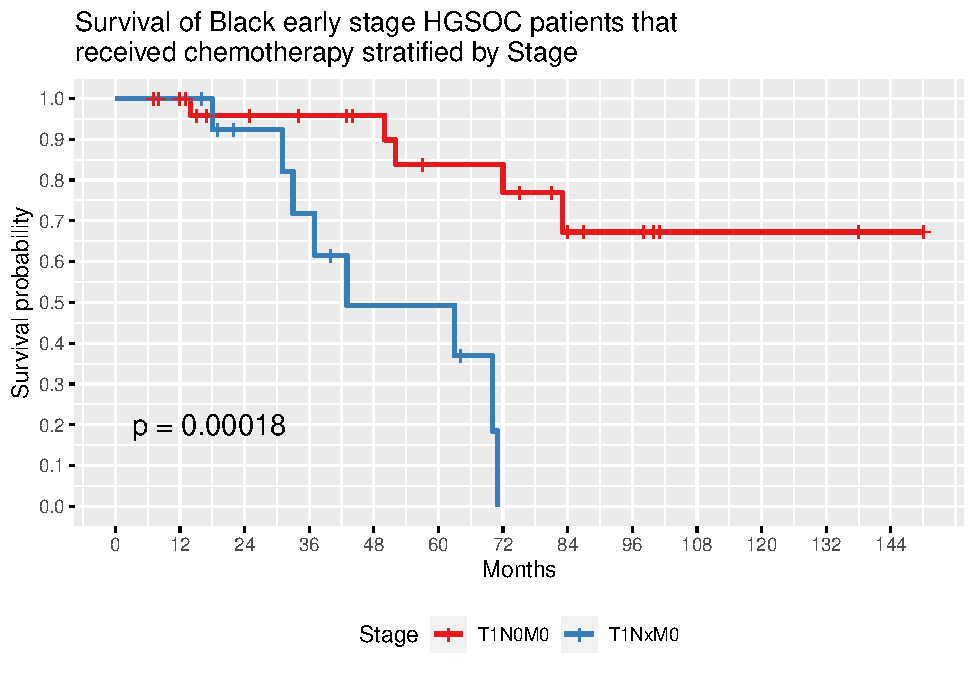
\includegraphics{EarlyOvaryRace_files/figure-latex/unnamed-chunk-8-1.pdf}

\begin{tabular}[t]{l|r}
\hline
Positive Nodes & Count\\
\hline
No & 28\\
\hline
Unk & 14\\
\hline
\end{tabular}

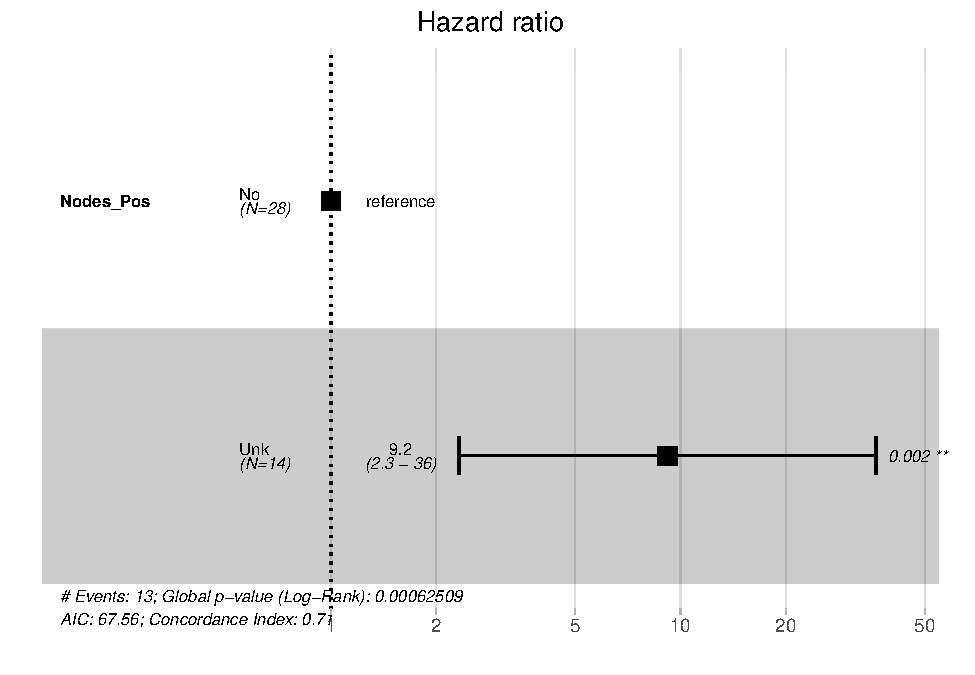
\includegraphics{EarlyOvaryRace_files/figure-latex/unnamed-chunk-9-1.pdf}

\begin{verbatim}
## Call:
## coxph(formula = Surv(SurvMonths, COD) ~ Nodes_Pos, data = HGS.ES.Black.Chemo)
## 
##   n= 42, number of events= 13 
## 
##               coef exp(coef) se(coef)     z Pr(>|z|)   
## Nodes_PosUnk 2.218     9.188    0.701 3.164  0.00156 **
## ---
## Signif. codes:  0 '***' 0.001 '**' 0.01 '*' 0.05 '.' 0.1 ' ' 1
## 
##              exp(coef) exp(-coef) lower .95 upper .95
## Nodes_PosUnk     9.187     0.1088     2.326      36.3
## 
## Concordance= 0.706  (se = 0.07 )
## Likelihood ratio test= 11.7  on 1 df,   p=6e-04
## Wald test            = 10.01  on 1 df,   p=0.002
## Score (logrank) test = 13.98  on 1 df,   p=2e-04
\end{verbatim}

\hypertarget{white-race}{%
\subsection{White Race}\label{white-race}}

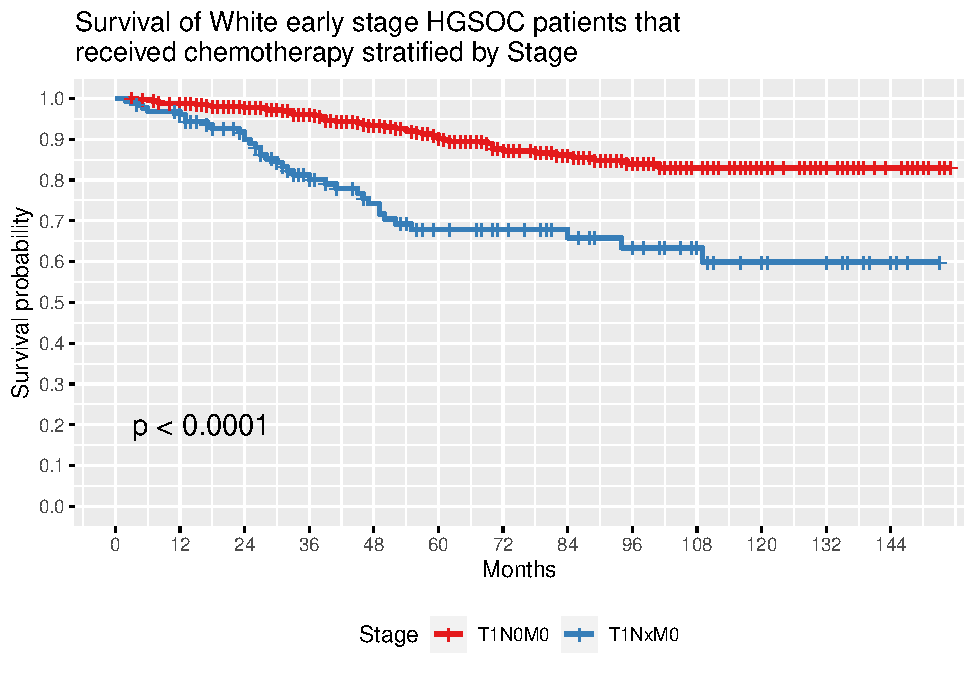
\includegraphics{EarlyOvaryRace_files/figure-latex/unnamed-chunk-10-1.pdf}

\begin{tabular}[t]{l|r}
\hline
Positive Nodes & Count\\
\hline
No & 454\\
\hline
Unk & 126\\
\hline
\end{tabular}

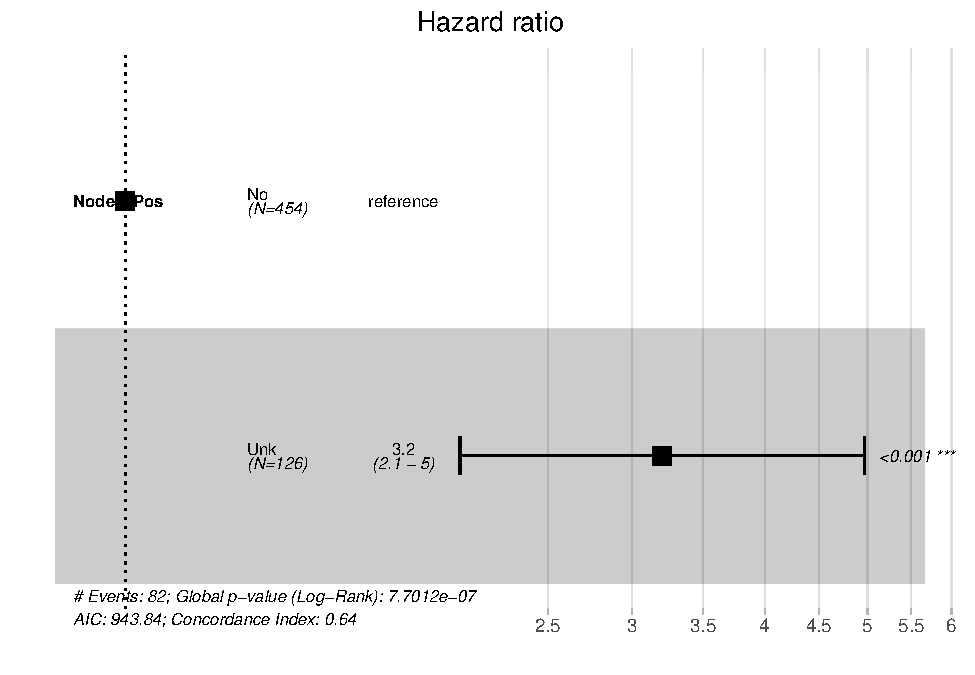
\includegraphics{EarlyOvaryRace_files/figure-latex/unnamed-chunk-11-1.pdf}

\begin{verbatim}
## Call:
## coxph(formula = Surv(SurvMonths, COD) ~ Nodes_Pos, data = HGS.ES.White.Chemo)
## 
##   n= 580, number of events= 82 
## 
##                coef exp(coef) se(coef)     z Pr(>|z|)    
## Nodes_PosUnk 1.1643    3.2036   0.2237 5.206 1.93e-07 ***
## ---
## Signif. codes:  0 '***' 0.001 '**' 0.01 '*' 0.05 '.' 0.1 ' ' 1
## 
##              exp(coef) exp(-coef) lower .95 upper .95
## Nodes_PosUnk     3.204     0.3122     2.067     4.966
## 
## Concordance= 0.637  (se = 0.028 )
## Likelihood ratio test= 24.43  on 1 df,   p=8e-07
## Wald test            = 27.1  on 1 df,   p=2e-07
## Score (logrank) test = 30.28  on 1 df,   p=4e-08
\end{verbatim}

\hypertarget{hispanic-race}{%
\subsection{Hispanic Race}\label{hispanic-race}}

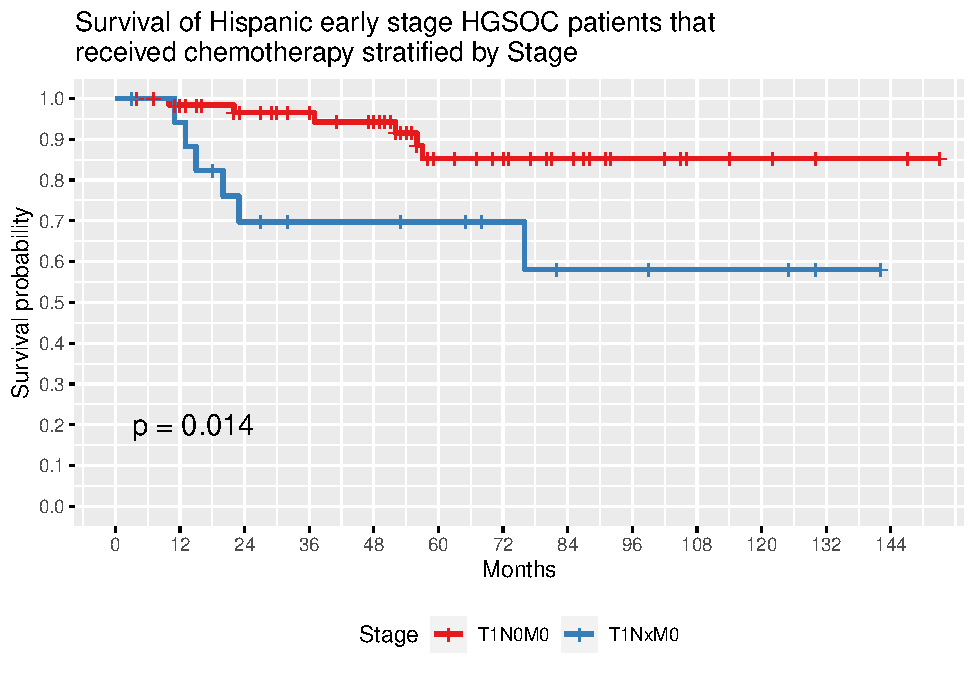
\includegraphics{EarlyOvaryRace_files/figure-latex/unnamed-chunk-12-1.pdf}

\begin{tabular}[t]{l|r}
\hline
Positive Nodes & Count\\
\hline
No & 63\\
\hline
Unk & 18\\
\hline
\end{tabular}

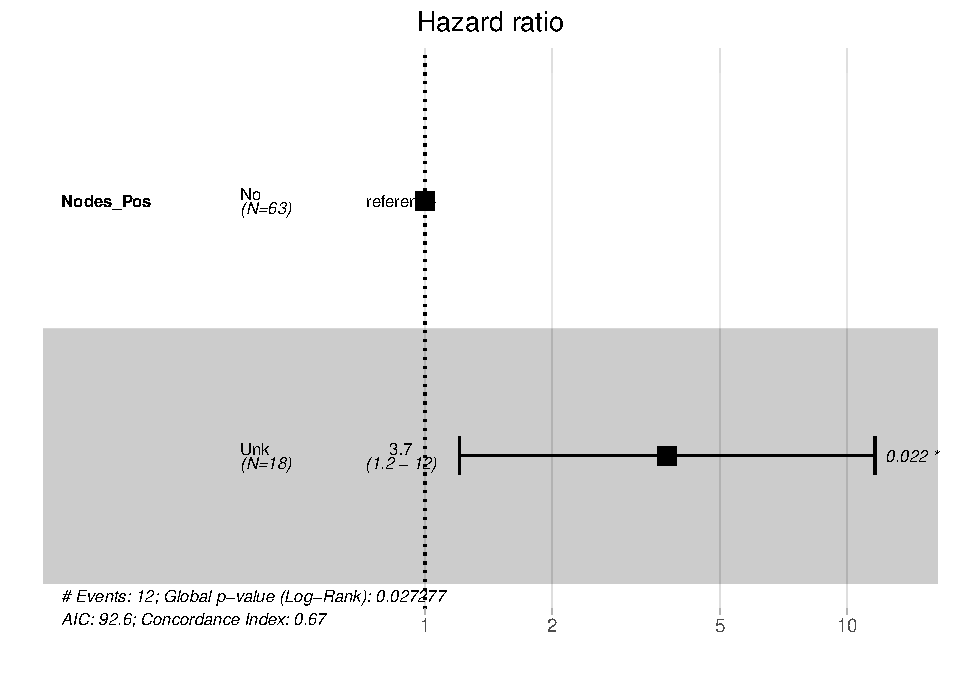
\includegraphics{EarlyOvaryRace_files/figure-latex/unnamed-chunk-13-1.pdf}

\begin{verbatim}
## Call:
## coxph(formula = Surv(SurvMonths, COD) ~ Nodes_Pos, data = HGS.ES.Hisp.Chemo)
## 
##   n= 81, number of events= 12 
## 
##                coef exp(coef) se(coef)     z Pr(>|z|)  
## Nodes_PosUnk 1.3209    3.7468   0.5787 2.282   0.0225 *
## ---
## Signif. codes:  0 '***' 0.001 '**' 0.01 '*' 0.05 '.' 0.1 ' ' 1
## 
##              exp(coef) exp(-coef) lower .95 upper .95
## Nodes_PosUnk     3.747     0.2669     1.205     11.65
## 
## Concordance= 0.67  (se = 0.074 )
## Likelihood ratio test= 4.87  on 1 df,   p=0.03
## Wald test            = 5.21  on 1 df,   p=0.02
## Score (logrank) test = 6  on 1 df,   p=0.01
\end{verbatim}

\hypertarget{does-use-of-chemotherapy-matter-by-stage-for-each-race}{%
\section{Does use of chemotherapy matter by stage for each
race?}\label{does-use-of-chemotherapy-matter-by-stage-for-each-race}}

\hypertarget{black-race-1}{%
\subsection{Black Race}\label{black-race-1}}

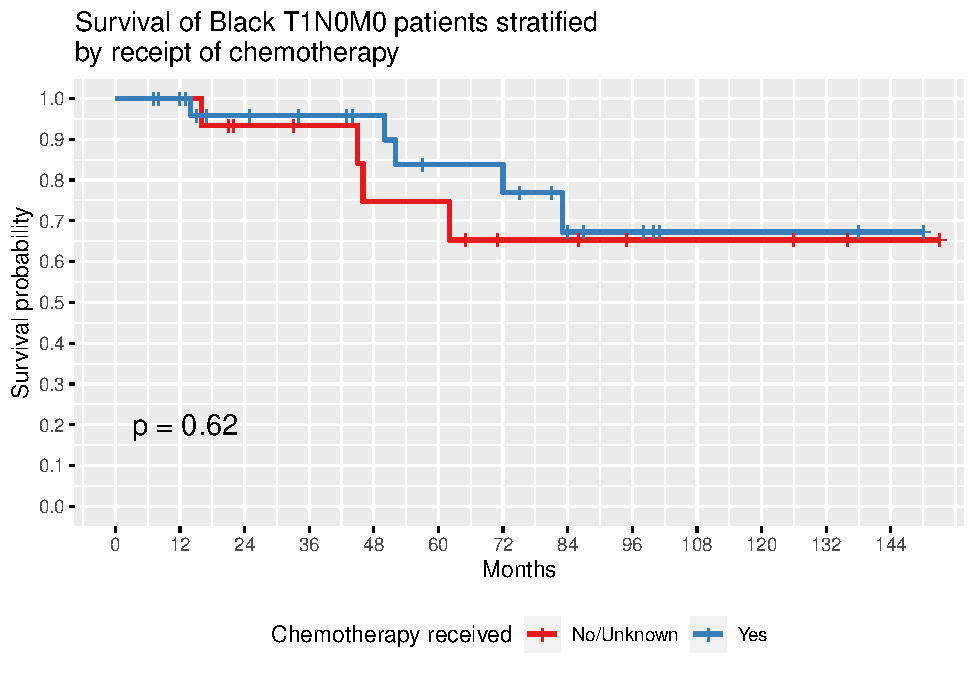
\includegraphics{EarlyOvaryRace_files/figure-latex/unnamed-chunk-14-1.pdf}

\begin{tabular}[t]{l|r}
\hline
Chemotherapy received & Count\\
\hline
No/Unknown & 15\\
\hline
Yes & 28\\
\hline
\end{tabular}

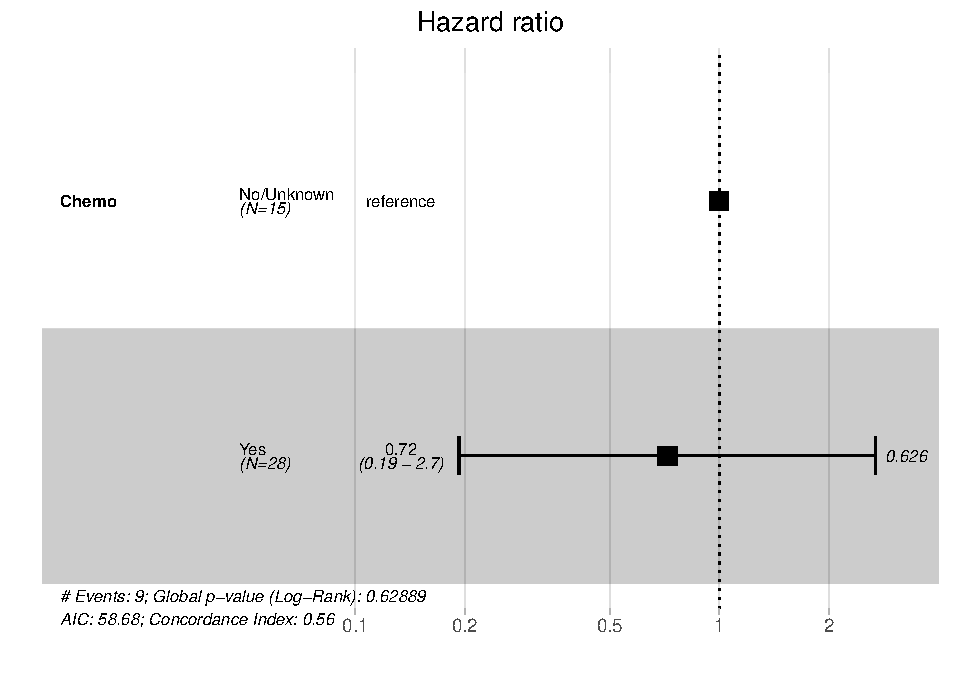
\includegraphics{EarlyOvaryRace_files/figure-latex/unnamed-chunk-15-1.pdf}

\begin{verbatim}
## Call:
## coxph(formula = Surv(SurvMonths, COD) ~ Chemo, data = HGS.Black.N0)
## 
##   n= 43, number of events= 9 
## 
##             coef exp(coef) se(coef)      z Pr(>|z|)
## ChemoYes -0.3277    0.7206   0.6726 -0.487    0.626
## 
##          exp(coef) exp(-coef) lower .95 upper .95
## ChemoYes    0.7206      1.388    0.1928     2.693
## 
## Concordance= 0.558  (se = 0.089 )
## Likelihood ratio test= 0.23  on 1 df,   p=0.6
## Wald test            = 0.24  on 1 df,   p=0.6
## Score (logrank) test = 0.24  on 1 df,   p=0.6
\end{verbatim}

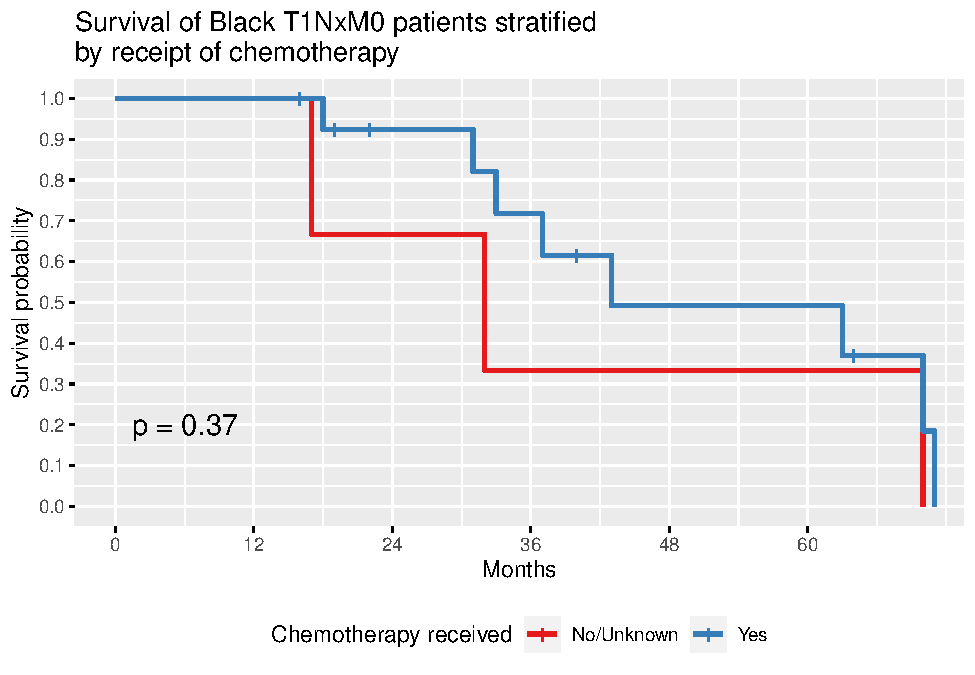
\includegraphics{EarlyOvaryRace_files/figure-latex/unnamed-chunk-16-1.pdf}

\begin{tabular}[t]{l|r}
\hline
Chemotherapy received & Count\\
\hline
No/Unknown & 3\\
\hline
Yes & 14\\
\hline
\end{tabular}

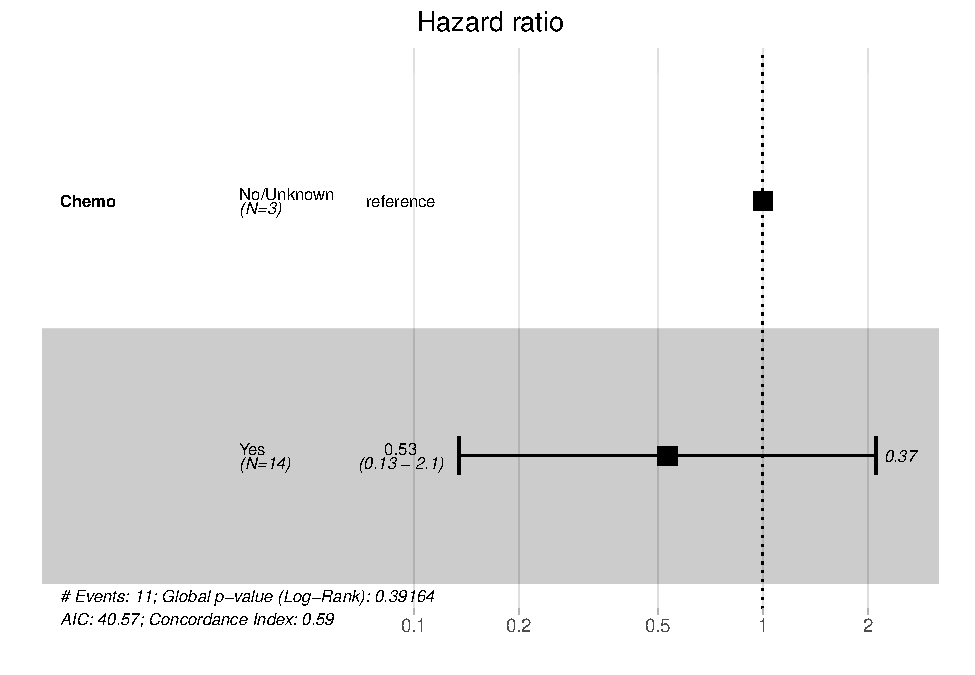
\includegraphics{EarlyOvaryRace_files/figure-latex/unnamed-chunk-17-1.pdf}

\begin{verbatim}
## Call:
## coxph(formula = Surv(SurvMonths, COD) ~ Chemo, data = HGS.Black.Nx)
## 
##   n= 17, number of events= 11 
## 
##             coef exp(coef) se(coef)      z Pr(>|z|)
## ChemoYes -0.6283    0.5335   0.7016 -0.896     0.37
## 
##          exp(coef) exp(-coef) lower .95 upper .95
## ChemoYes    0.5335      1.874    0.1349      2.11
## 
## Concordance= 0.595  (se = 0.095 )
## Likelihood ratio test= 0.73  on 1 df,   p=0.4
## Wald test            = 0.8  on 1 df,   p=0.4
## Score (logrank) test = 0.83  on 1 df,   p=0.4
\end{verbatim}

\hypertarget{white-race-1}{%
\subsection{White Race}\label{white-race-1}}

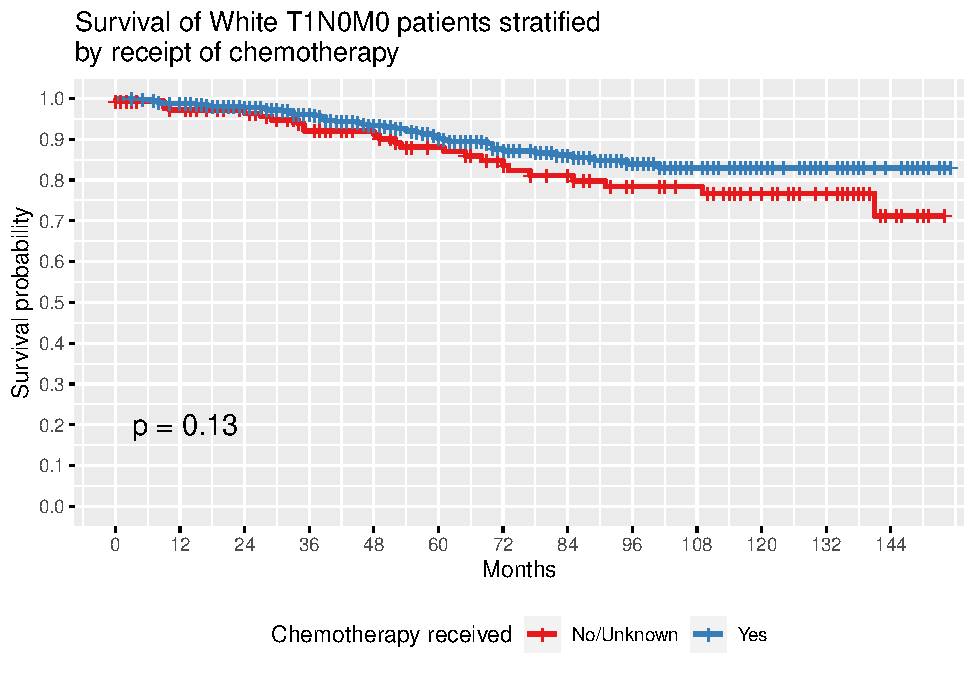
\includegraphics{EarlyOvaryRace_files/figure-latex/unnamed-chunk-18-1.pdf}

\begin{tabular}[t]{l|r}
\hline
Chemotherapy received & Count\\
\hline
No/Unknown & 144\\
\hline
Yes & 454\\
\hline
\end{tabular}

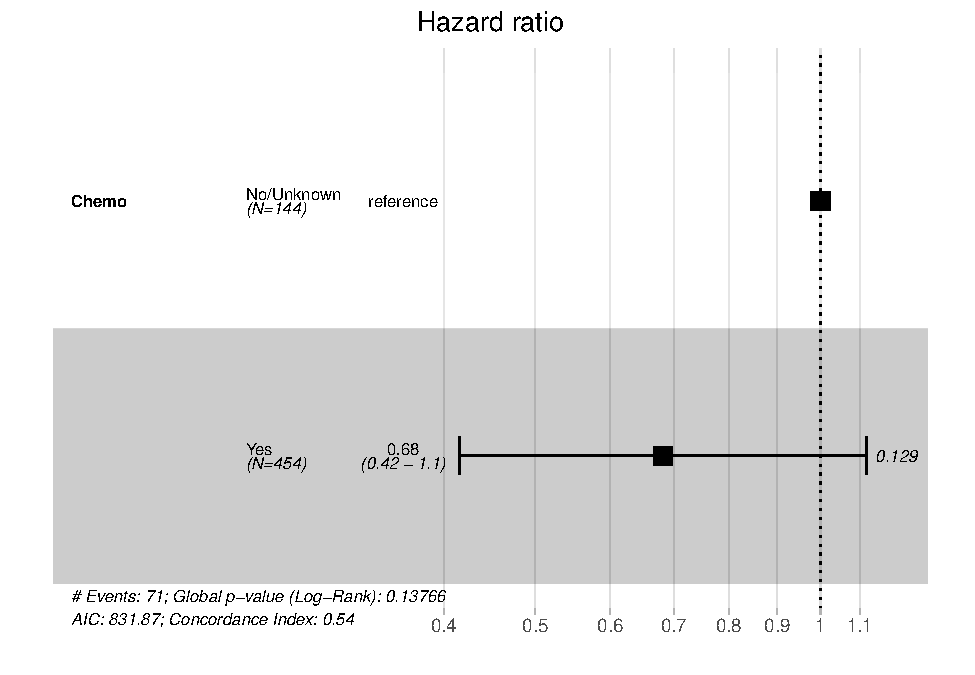
\includegraphics{EarlyOvaryRace_files/figure-latex/unnamed-chunk-19-1.pdf}

\begin{verbatim}
## Call:
## coxph(formula = Surv(SurvMonths, COD) ~ Chemo, data = HGS.White.N0)
## 
##   n= 598, number of events= 71 
## 
##             coef exp(coef) se(coef)      z Pr(>|z|)
## ChemoYes -0.3828    0.6820   0.2521 -1.519    0.129
## 
##          exp(coef) exp(-coef) lower .95 upper .95
## ChemoYes     0.682      1.466    0.4161     1.118
## 
## Concordance= 0.538  (se = 0.029 )
## Likelihood ratio test= 2.2  on 1 df,   p=0.1
## Wald test            = 2.31  on 1 df,   p=0.1
## Score (logrank) test = 2.33  on 1 df,   p=0.1
\end{verbatim}

\includegraphics{EarlyOvaryRace_files/figure-latex/unnamed-chunk-20-1.pdf}

\begin{tabular}[t]{l|r}
\hline
Chemotherapy received & Count\\
\hline
No/Unknown & 71\\
\hline
Yes & 126\\
\hline
\end{tabular}

\includegraphics{EarlyOvaryRace_files/figure-latex/unnamed-chunk-21-1.pdf}

\begin{verbatim}
## Call:
## coxph(formula = Surv(SurvMonths, COD) ~ Chemo, data = HGS.White.Nx)
## 
##   n= 197, number of events= 56 
## 
##              coef exp(coef) se(coef)    z Pr(>|z|)
## ChemoYes -0.05535   0.94615  0.27660 -0.2    0.841
## 
##          exp(coef) exp(-coef) lower .95 upper .95
## ChemoYes    0.9461      1.057    0.5502     1.627
## 
## Concordance= 0.516  (se = 0.035 )
## Likelihood ratio test= 0.04  on 1 df,   p=0.8
## Wald test            = 0.04  on 1 df,   p=0.8
## Score (logrank) test = 0.04  on 1 df,   p=0.8
\end{verbatim}

\hypertarget{hispanic}{%
\subsection{Hispanic}\label{hispanic}}

\includegraphics{EarlyOvaryRace_files/figure-latex/unnamed-chunk-22-1.pdf}

\begin{tabular}[t]{l|r}
\hline
Chemotherapy received & Count\\
\hline
No/Unknown & 20\\
\hline
Yes & 63\\
\hline
\end{tabular}

\includegraphics{EarlyOvaryRace_files/figure-latex/unnamed-chunk-23-1.pdf}

\begin{verbatim}
## Call:
## coxph(formula = Surv(SurvMonths, COD) ~ Chemo, data = HGS.Hisp.N0)
## 
##   n= 83, number of events= 8 
## 
##             coef exp(coef) se(coef)    z Pr(>|z|)
## ChemoYes 0.04951   1.05076  0.81854 0.06    0.952
## 
##          exp(coef) exp(-coef) lower .95 upper .95
## ChemoYes     1.051     0.9517    0.2112     5.227
## 
## Concordance= 0.516  (se = 0.072 )
## Likelihood ratio test= 0  on 1 df,   p=1
## Wald test            = 0  on 1 df,   p=1
## Score (logrank) test = 0  on 1 df,   p=1
\end{verbatim}

\includegraphics{EarlyOvaryRace_files/figure-latex/unnamed-chunk-24-1.pdf}

\begin{tabular}[t]{l|r}
\hline
Chemotherapy received & Count\\
\hline
No/Unknown & 10\\
\hline
Yes & 18\\
\hline
\end{tabular}

\includegraphics{EarlyOvaryRace_files/figure-latex/unnamed-chunk-25-1.pdf}

\begin{verbatim}
## Call:
## coxph(formula = Surv(SurvMonths, COD) ~ Chemo, data = HGS.Hisp.Nx)
## 
##   n= 28, number of events= 9 
## 
##            coef exp(coef) se(coef)     z Pr(>|z|)
## ChemoYes 0.3245    1.3834   0.7123 0.456    0.649
## 
##          exp(coef) exp(-coef) lower .95 upper .95
## ChemoYes     1.383     0.7229    0.3425     5.587
## 
## Concordance= 0.607  (se = 0.057 )
## Likelihood ratio test= 0.21  on 1 df,   p=0.6
## Wald test            = 0.21  on 1 df,   p=0.6
## Score (logrank) test = 0.21  on 1 df,   p=0.6
\end{verbatim}

\hypertarget{overall-coxph-and-forest-plot}{%
\section{Overall CoxPH and Forest
plot}\label{overall-coxph-and-forest-plot}}

\includegraphics{EarlyOvaryRace_files/figure-latex/unnamed-chunk-26-1.pdf}

\begin{verbatim}
## Call:
## coxph(formula = Surv(SurvMonths, COD) ~ TNM.Stage + Lat + Chemo + 
##     Race.Group + LND, data = HGS.ES)
## 
##   n= 1052, number of events= 177 
## 
##                         coef exp(coef)  se(coef)      z Pr(>|z|)    
## TNM.StageT1NxM0     1.158405  3.184850  0.176442  6.565 5.19e-11 ***
## LatLeft            -0.164370  0.848428  0.189861 -0.866 0.386635    
## LatRight           -0.083209  0.920159  0.191995 -0.433 0.664732    
## LatUnknown          0.118951  1.126314  0.526900  0.226 0.821392    
## ChemoYes           -0.153641  0.857580  0.160357 -0.958 0.338002    
## Race.GroupHispanic -0.005811  0.994206  0.259451 -0.022 0.982132    
## Race.GroupBlack     0.927706  2.528703  0.243005  3.818 0.000135 ***
## Race.GroupOther    -0.001817  0.998185  0.294047 -0.006 0.995070    
## LNDInadequate       0.195856  1.216351  0.207715  0.943 0.345729    
## LNDNone                   NA        NA  0.000000     NA       NA    
## ---
## Signif. codes:  0 '***' 0.001 '**' 0.01 '*' 0.05 '.' 0.1 ' ' 1
## 
##                    exp(coef) exp(-coef) lower .95 upper .95
## TNM.StageT1NxM0       3.1848     0.3140    2.2537     4.501
## LatLeft               0.8484     1.1787    0.5848     1.231
## LatRight              0.9202     1.0868    0.6316     1.341
## LatUnknown            1.1263     0.8879    0.4010     3.163
## ChemoYes              0.8576     1.1661    0.6263     1.174
## Race.GroupHispanic    0.9942     1.0058    0.5979     1.653
## Race.GroupBlack       2.5287     0.3955    1.5705     4.071
## Race.GroupOther       0.9982     1.0018    0.5609     1.776
## LNDInadequate         1.2164     0.8221    0.8096     1.828
## LNDNone                   NA         NA        NA        NA
## 
## Concordance= 0.667  (se = 0.021 )
## Likelihood ratio test= 63  on 9 df,   p=4e-10
## Wald test            = 68.56  on 9 df,   p=3e-11
## Score (logrank) test = 75.54  on 9 df,   p=1e-12
\end{verbatim}

\begin{verbatim}
##              chisq df     p
## TNM.Stage   4.6037  1 0.032
## Lat         3.6356  3 0.304
## Chemo       0.0854  1 0.770
## Race.Group  4.3033  3 0.231
## LND         0.8886  1 0.346
## GLOBAL     17.6237  9 0.040
\end{verbatim}

\includegraphics{EarlyOvaryRace_files/figure-latex/unnamed-chunk-27-1.pdf}

\end{document}
